\documentclass[12pt]{article}
\usepackage{pgf, tikz}
\usepackage{amsmath, amsfonts, amssymb, graphicx}
\usepackage{subfig}
\usepackage{float}
\usepackage{algorithm, caption}
\usepackage[noend]{algpseudocode}
\usepackage[utf8]{inputenc}
\usepackage[spanish]{babel}
\usepackage{amsthm}

\setlength{\textheight}{23cm} \setlength{\evensidemargin}{0cm}
\setlength{\oddsidemargin}{-.5cm} \setlength{\topmargin}{-3cm}
\setlength{\textwidth}{17.5cm} \setlength{\parskip}{.2cm}


%opening

\begin{document}
	\begin{picture}(80, 80)
	\put(170,0){\hbox{
\includegraphics[scale=0.6]{cimat_logo.png}}}
	\end{picture}
	
	\begin{center}
		\begin{huge}
			Centro de Investigación en Matemáticas, A.C.
		\end{huge}
	\end{center}

	\begin{center}
		\begin{large}
			Reporte tarea 6 - Programación y algoritmos
		\end{large}
	\end{center}
	
	\begin{center}
		\textbf{Erick Salvador Alvarez Valencia}
	\end{center}

	\begin{center}
		25 de Septiembre de 2017
	\end{center}



%\maketitle

%\tableofcontents

\section{Resumen}
Este reporte se describirá el avance semanal del clasificador de textos, en esta ocasión se desarrolló un generador de vectores binarios, en el cual, mediante el algoritmo $UMDA$ se realizan muchas generaciones de vectores binarios y se irán tomando las mejores poblaciones, a la par que se actualiza un vector de probabilidades, el cual nos sirve para seguir generando las poblaciones.\\
Finalmente se hablará un poco sobre la generación de un archivo $Makefile$ el cual se usa para compilar el presente proyecto, de la misma forma contiene más opciones.

\section{Desarrollo}
Primeramente hay que recordar que en la entrega pasada, donde se añadieron las estructuras para la clasificación, se modificó el generador de textos, el cual ahora genera bloques de 5000 palabras en lugar de 5000 caracteres. Posteriormente se procedió a implementar un algoritmo que obtiene las mejores $N$ palabras de la matriz de frecuencias. Dicho algoritmo se presenta a continuación:\\

\begin{algorithm}[H]
\caption{Algoritmo para obtener las $N$ mejores palabras.}
\begin{algorithmic}[1]
\Procedure{GetBestWords}{$Frec, N, NBloques$}
\State $Table\gets$ Tabla que almacena el Id y la Frecuencia.
\State $Table\gets$ Dar memoria al objeto.
\For{$i\gets 1\ to\ n$}
\State $Sum$ = $0$
\For{$j\gets 1\ to\ NBloques$}
\State $Sum$ = $Frec[i][j]$
\EndFor
\State Añadir el índice y $Sum$ a $Table_i$
\EndFor
\State Ordenar $Table$
\State $FrecRes\gets$ Matriz con $N$ filas y $NBloques$ columnas.
\State Copiar $Table$ a $FrecRes$
\State \textbf{return} $FrecRes$
\EndProcedure
\end{algorithmic}
\end{algorithm}

Posteriormente se realizó la implementación del algoritmo $UMDA$ la cual consiste en lo siguiente:\\
Se genera un objeto con todo lo necesario para realizar la clasificación con la matríz de las $N$ mejores palabras, ahora necesitamos una función que genere un vector binario en función de un vector de probabilidades $P$, llamemos $GenerarYReparar$ a esa función, la cual recibe de entrada el vector de probabilidades, el tamaño de dicho vector y el número de 1's que debe tener el vector binario de salida. 

Una vez se tiene definida la función anterior se puede proceder a generar los vectores. Primero definimos $Npop$ el número de vectores binarios que se harán por generación, $Niter$ el número de iteraciones en caso de que no converga las nuevas generaciones, $t$ la iteración actual, y $X^t$ la matríz de vectores binarios en el tiempo $t$. Inicialmente el vector de probabilidades $P$ el cual es de tamaño $N$, tiene sus valores inicializados en $0.5$, lo cual nos indica que la probabilidad de generar un $1$ en la iésima posición del vector binario es del $50\%$.\\

El algoritmo se repite mientras no se cumpla alguna condición de paro, existen tres condiciones, las cuales son: que la norma del vector $P$ sea mejor a $N/4$, que se cumplan las $t$ iteraciones y que se encuentre un vector que genere la mejor métrica posible. Ahora, en la iteración $t$ se tiene que generar la matriz $X^t$ tenemos que llamar a la función $GenerarYReparar$ $Npop\ -\ 1$ veces, esto porque al menos debemos conservar el mejor vector de la generación anterior, inicialmente si llenamos este vector con la función anterior ya que no disponemos de una generación anterior. Ahora por cada vector $X_i$ debemos realizar la clasificación usando el objeto que ya tenemos preparado y se tiene que ir guardando las métricas obtenidas, al finalizar la serie de clasificaciones debemos ordenar las métricas, esto para saber a qué vectores binarios se refieren las más grandes. El paso siguiente es guardar el vector con la mejor probabilidad en la variable $xBest$ y de la misma forma en la matriz $X$, posterior a eso se actualiza el vector $P$, la idea es que cada nueva posición de $P_i$ se obtiene de sacar el promedio con la iésima columna de la matriz $X$, pero hay que tener en cuenta que solo tomamos la mitad de la misma, osea $Npop/2$. Después de esto volvemos al paso uno para generar la siguiente población.\\
EL pseudocódigo de este algoritmo no se muestra ya que fue provisto en la descripción de la tarea.

\section{Pruebas realizadas}
Se realizaron varias pruebas al problema, donde se cambiaron los parámetros $Nfeat$ y $Npop$ mayoritariamente, donde los resultados obtenidos variaron en muchos ámbitos, desde la forma en que finalizaba el algoritmo, en algunas ocasiones se detenía porque se cumplía el número de iteraciones, en otras se encontraba el mejor vector y en otras se cumplía la convergencia en la norma. Para demostrar esto se incluye una captura de pantalla de una ejecución que se realizó con una semilla predeterminada:\\

\begin{figure}[H]
	\centering
	\subfloat[][Figura 1. Resultado de la ejecución del programa con una semilla predefinida.]{
		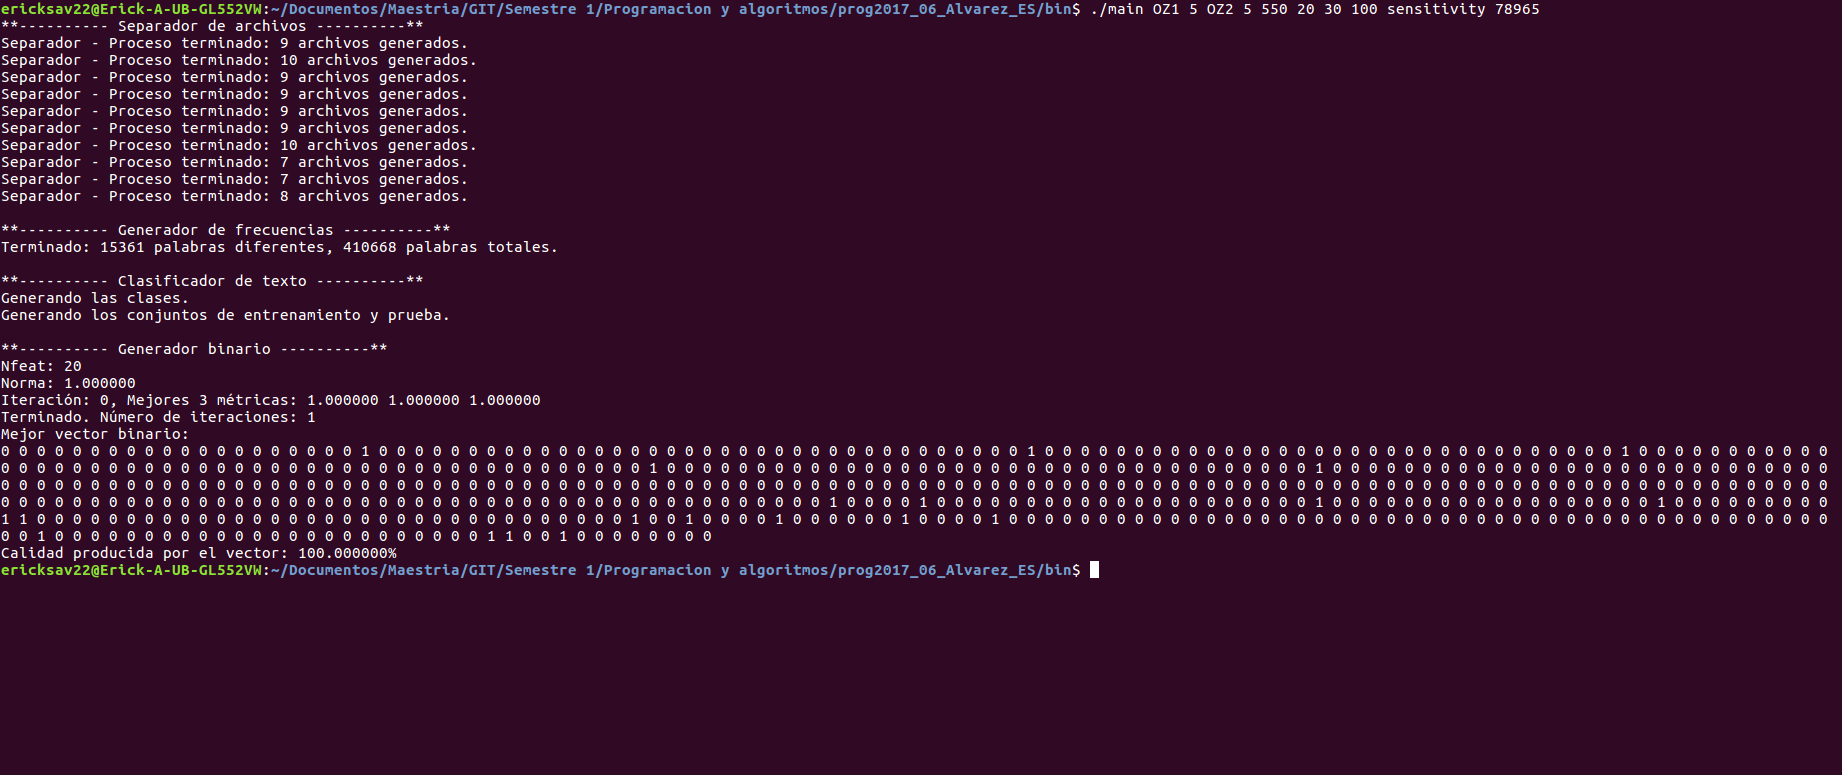
\includegraphics[scale=0.2]{E1.png}
	}\hfill
\end{figure}

En este ejemplo se encontró el mejor vector binario en una sola iteración, esto debido a que el valor de $Nfeat$ es considerable.

\section{Conslusiones}
Se concluye que el programa trabajó de una forma correcta, no siempre se encontraba el mejor vector binario, dependiendo de los parámetros de entrada, una mejora podría ser alguna optimización estocástica o heurística, cabe destacar que el mismo programa se corrió bajo valgrind y no presentó fugas de memoria.\\

Otra cosa que se debe decir es que se realizó un archivo Makefile el cual permite compilar este software de diferentes maneras, así como el presente reporte, y también limpiar los archivos generados bajo las compilaciones y las ejecuciones.
\end{document}
